
\section{Merging}\label{sec:merging}
In this section we will define some approaches and heuristics in order to solve MAPF problems given a \(\tau\) input. The expression ``solving a conflict'' (or similar) will occurs, it however do not represent anything formal; it represent a moment where an approach has a solution to reach a vertex that is after the conflicting vertex, in the sequence of vertices \(pi\). Thus, it does not mean that no conflict may occurs because of the resolution.




\subsection{Sub-graphs}\label{sec:subgraphs}
Approaches in this section are using sub-graphs; one sub-graph is a graph based on \(G\) with the scope of a set of paths \(\gamma\); for every \(\gamma\) in \(\tau\) we have an associated sub-graph \(\mathcal{S}(\gamma)\). In others words, \(n\) agents result in \(n\) sub-graphs. For instance, let an agent \(a_{red}\) and \(a_{blue}\) with their set of paths \(\gamma_{red}\) and \(\gamma_{blue}\) where \(|\gamma_{red}| = 2\) and \(|\gamma_{blue}| = 1\). The result of the decomposition of \(\tau\) in sub-graphs is in figure~\ref{img:from_graph}. 

\begin{figure}[H]
  \centering
  \caption{Decomposition of \(\tau\) in sub-graphs }\label{img:from_graph}
  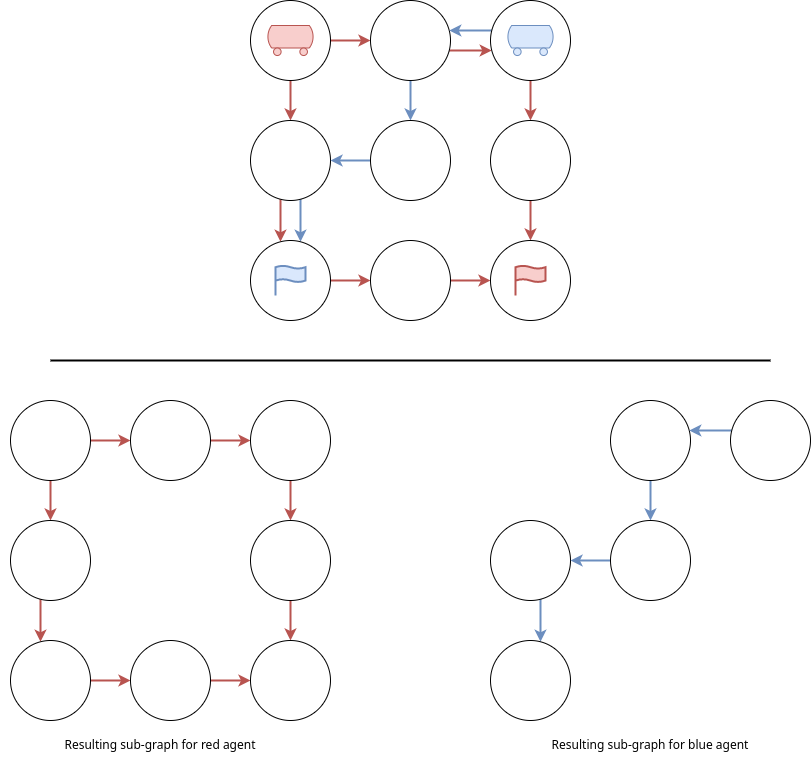
\includegraphics[width=\widthimg]{img/from_graph_to_subgraph.drawio.png}
\end{figure}

Sub-graphs by themselves are not useful, approaches can extend the sub-graphs according to strategies. Intuitively, an ``extension'' represent additional possibilities in order to solve a conflict. 

\subsubsection{Witness solver}

In this section, we will introduce a witness solver; a witness solver (WS) will be the basic solver that aims to solve MAPF instance given a \(\tau\) input. It works as such; it converts the input \(\tau\) in a set of \(n\) graph that are sub-graph of \(G\) as described in section~\ref{sec:subgraphs}. We then have two cases: there is a valid plan made out from \(\tau\) that contains no path-conflict, or there is no valid plan that can be build ot of \(\tau\) directly. In the first case, the merging process will give the valid plan as output, in the second case, the WS will try to solve the instance by using different approaches, strategies or heuristics until finding a valid set of paths that is a valid plan.

The first case occurs if it exists a set \(\{pick(\gamma) | \gamma \in \tau\}\) which correspond to a collection of path, is conflict-free, we refer to this case as ``straightforward solving''. 

\subsubsection{Corridor}\label{sec:corridor}

The corridor approach aims to help the solving process by extending the size of the sub-graph generated by a set of path \(\gamma\). It extends the sub-graph by adding to the sub-graph the direct neighbor vertices (and their associated edges). Applying the corridor extension successively \(x\) times will result of a corridor of level \(x\) for instance:  
\begin{figure}[H]
  \centering
  \caption{Example of corridor}\label{img:corridor}
  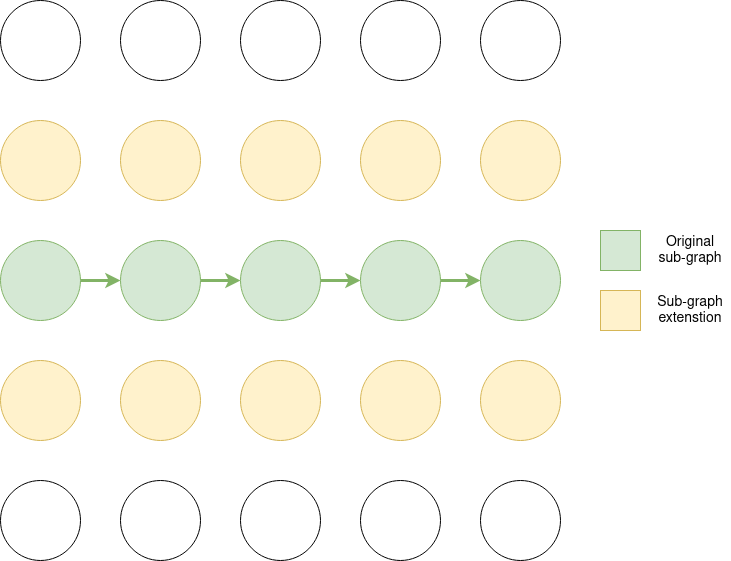
\includegraphics[width=\widthimg]{img/corridor.drawio}
\end{figure}

We can define corridor as such;

\[
 corridor(s,(V,E)) = \{v' | v' \in V, v\in s, (v,v') \in E \}
\] where s represent of set of vertices.

A corridor of \(k\)-level(s) is obtained by recursively use the corridor function \(k\) time on its output: e.g. \(corridor(corridor(vertex(\pi),G))\) represent a 2-levels corridor.
We can assume some elements about this approach; with a big enough \(k\) size the whole graph is covered. Using the witness solver would end up doing classic MAPF. Furthermore for large instances, a huge part of the extension would probably not be used ending up adding more space search for the witness solver. We can also identify instances where corridor extension would be probably interesting to use when the ``dodge'' movement required to solve a conflicts is situated in the graph ``far away'' (a distance relatively high) from where the conflict occurred. We can also assume that a set of distant paths would be an interesting set to work with; it potentially limits the number of ``overlapping'' vertices that would be added by the extension, see example shown in figure~\ref{img:case_corridor}. Also, corridors may work better on low density instances and low number of conflicts and potential conflict since it is not adding so much depth of possible movement.

In practice, we can create corridor only for path that have a path conflict, we can also choose to create corridor only for one of the two agent involved in a conflict.


\begin{figure}[H]
  \centering
  \caption{Most Distant paths and corridor extension}\label{img:case_corridor}
  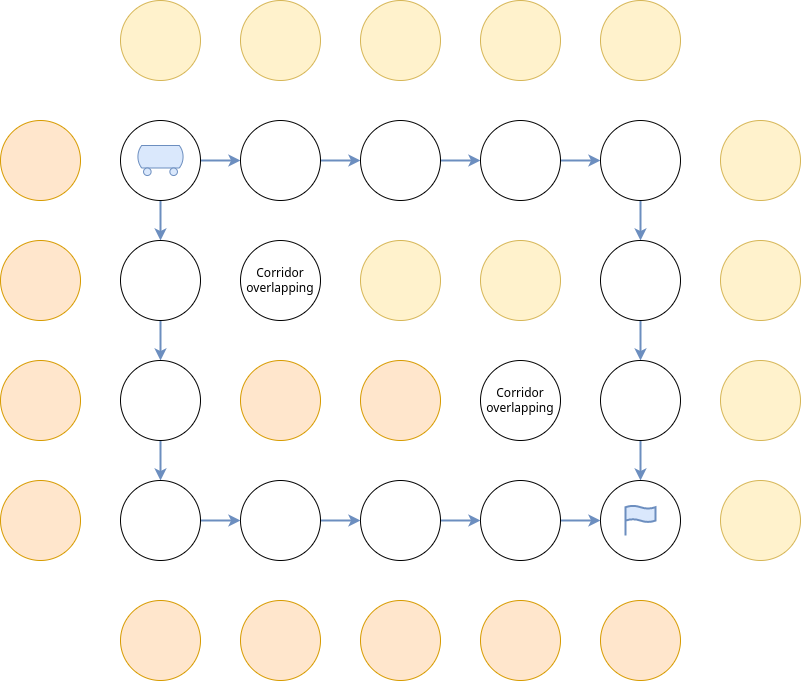
\includegraphics[width=\widthimg]{img/case_corridor.drawio.png}
\end{figure}


\subsubsection{Diamond extention}

The diamond extension aims to extend the sub-graph by adding diamonds of vertices around potential conflict or plan conflict. As shown in figure~\ref{img:diamond}, we can se different levels of diamond extension which will increase the size of the sub-graph, by extension the possibilities in order to solve the conflict.
\begin{figure}[H]
  \centering
  \caption{Example of diamond of size 1 and 2}\label{img:diamond}
  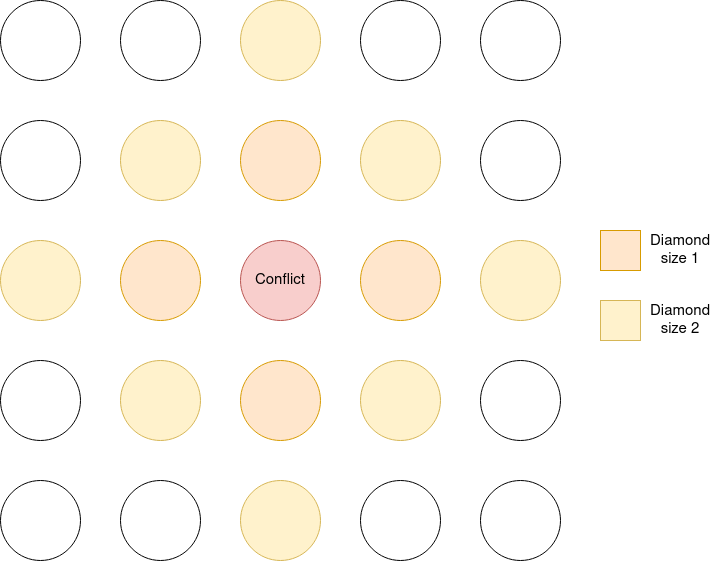
\includegraphics[width=\widthimg]{img/diamond.drawio.png}
\end{figure}

As described for the corridor instance, having a \(k\) as diamond size too big would end up covering the whole graph. This approach would probably works fine with a relatively small \nameref{sec:conflict_window}; having all conflicts concentrated in area of the graph would allow small size of the diamond extension, which reduce the space search. The instance represented in figure~\ref{img:diamond_case}, has a ``small'' conflict-window. While solving this instance (or this kind of instance, lot of robots, small conflict window) we can easily imagine that solving the conflicts issued by the IPF would create other conflicts but still in the same area. In consequences, diamond extension seems appropriate since the extension is covering also close area around conflicts. 
\begin{figure}[H]
  \centering
  \caption{Example of diamond extension interesting case }\label{img:diamond_case}
  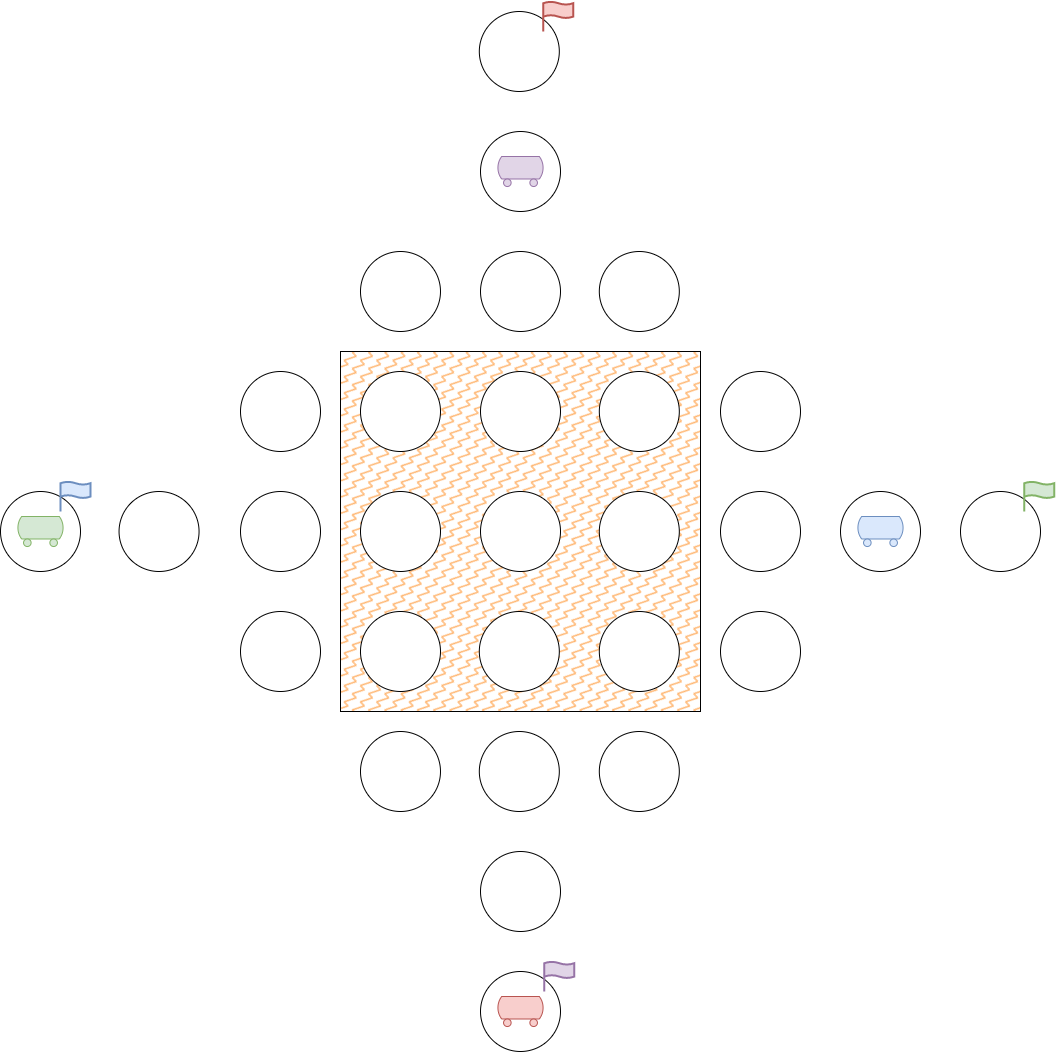
\includegraphics[width=7cm]{img/diamond_extension_case_example.drawio.png}
\end{figure}

From the properties described in section~\ref{sec:ipf}, we can argue that paths that have few bendings would work better for the diamond extension; a higher proportion of the extension (of size higher than 1) will already be in the original paths. Furthermore contrary to the corridor extension, whenever the proportion of conflict is low compared to the length of the path, diamond extension would probably work better e.g. figure\ref{img:diamond_vs_corridor}, based on section~\ref{sec:corridor} and figure~\ref{img:corridor} the proportion of the sub-graph that is not used is way higher for the diamond extension.

\begin{figure}[H]
  \centering
  \caption{Example of case where diamond extension would work but not corridor extension}\label{img:diamond_vs_corridor}
  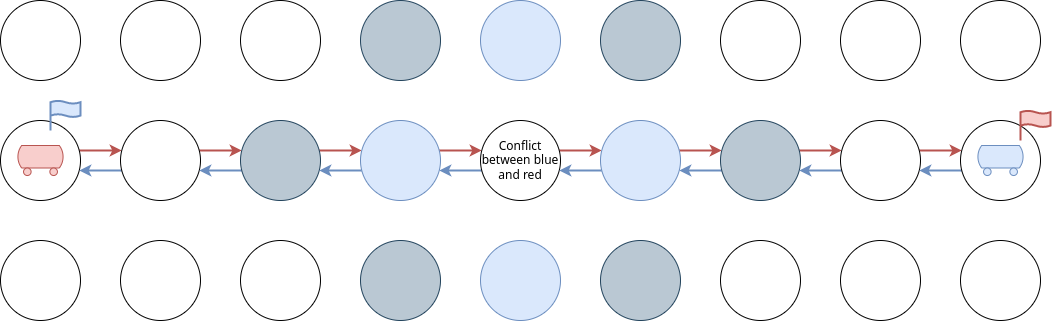
\includegraphics[width=\widthimg]{img/diamond_vs_corridor.drawio.png}
\end{figure}





\subsubsection{Systematic extention}

Approach presented above are not complete and aim to reduce the space search or computation time at the probable cost of optimality. Furthermore we can imagine instances where both approaches would not work, or require too much computation time. In the case represented on figure~\ref{img:systemetic_instance}, considering that \(\tau\) contains for both agent one shortest path, it is easy to tell that both heuristics on this kind of instances would not work decently because it would require that the extension covers the whole graph.

\begin{figure}[H]
  \centering
  \caption{Example instance that are more complex to solve}\label{img:systemetic_instance}
  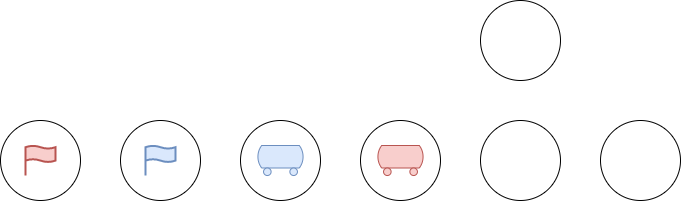
\includegraphics[width=\widthimg]{img/systematic_instance.drawio.png}
\end{figure}

We can use solving strategies described in paper~\cite{husvobbass22a,husvobbass22b}. These paper introduce four different strategies; Baseline Strategy,  Makespan-add Strategy, Prune-and-cut strategy and the Combined strategy. For short, these strategies are using a \(k-restricted graph\) which is similar to sub-graph; it takes a shortest path \(SP\) to define a subgraph, it also add ``vertices that are at most distance \(k\) away from some vertex in \(SP\)". The main idea is to add vertices and/or raise the makespan and see if a solution exist. According to the benchmarks, the Combined strategy seems to to most successful.




% \subsection{Guiding the agents}

% We described above strategies working with sub-graphs, however we can use \(\tau\) in other way. Instead of creating subgraph, we can uses all of the paths in \(\tau\) to create a ``heatmap''. Heatmap describe where agents has the most probable position. To do so, we project the probability of presence on each nodes of the graph for each time step. We can define two types of heatmaps, a ``global heatmap'', which refer to the heatmap considering all agents. And one specific to an agent, called ``local'' heatmap, respectively, we have  \(Heat(\tau)\) and \(heat(\gamma_a)\). We can define local as such:

% \[
%  heat(\gamma) = 
% \]

% Global heatmap is made of all local ones; in other words, for each nodes of the graph, we sum the probability of presence for each agent, the total being divided by the number of agents. There is some properties that we can infer from the global heatmap: if a node has a joined presence probability \(P\) of 1, we can tell that \(\tau\) contains no selection of paths for each agent such as no conflict occurs. This event is a specific case of a more general definition:

% \begin{definition}
%   If there is a vertex  \(v \in V\) having a \(P(v) \geq  1-(1/|A|)\), where \(P(v)\) is computed given an input \(\tau\), it is not possible select a path \(\pi\) where \(v \in \pi\) for straight forward solving.   
% \end{definition}

% (need a proof)








% The approach of heatmap uses the different path in \(\tau\) to project on graph the probability of presence of an agent. The figure~\ref{img:heatmap} shows the heat map of a graph considering \(\tau\) with two agents; a red one with two paths and a blue one with one path. 



% Using these ``probability of presence'' we can select which path to select to, in this case reduce


\section{Heatmap}

Based on paper \cite{atstfestko20a}

Heatmap is about projecting likelihood of presence of agents on vertices. Likelihood refers to the chance of an agent to be positioned at a specific vertex of the graph at a time step \(t\). We introduce \(\phi(a,v,t)\) which compute likelihood of the vertex \(v\) at time step \(t\) for the agent \(a\). 
To do so, we introduce a set \(P\) that is created as such : \[
  P = \bigcup^{a\in A}{}
\]
 From this definition, we can compute the first three step of an agent with an associated \(|\gamma|=3\) below (figure~\ref{img:heatmap}).

\begin{figure}[H]
  \centering
  \caption{Heatmap example of the first three time step for a \(|\gamma|=3\) }\label{img:heatmap}
  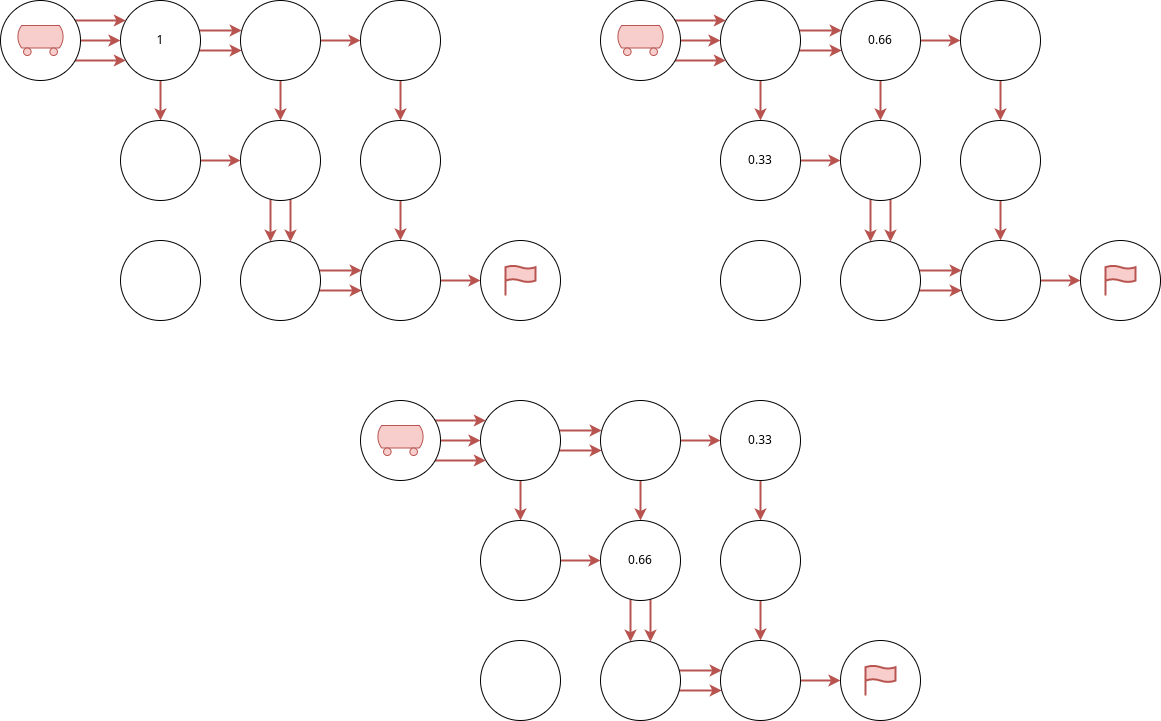
\includegraphics[width=12cm]{img/heatmap.drawio.png}
\end{figure}

This heatmap-per-agent can be used to compute a ``global one'', to do so, for each vertex and for each time step, we sum each \(\phi\) and then divide it by the number of agent (see appendix~\ref{apx:heatmap_and_global}), we will refer to this as \(\Phi\) where \(\Phi(v)\) refer to the value of a vertex \(v\). Computed this way, global heatmap do not represent likelihood of presence anymore but more of an indicator\footnote{I believe that we can find a way to compute global heatmap that could give us directly if the resolution is possible straightforward} where both heatmap taken together can be useful on different part of plan merging resolution.

\subsection{Heatmap as a property}


The heatmap we proposed is from the perspective of agents, but it can also be considered with regards to the \(\gamma\)'s scope. To do so we define the following sequence (which is not modifying the computation of heatmap)
\[
  fun(\pi_a) = \{(v,\phi(a,v,t))| (v,t) \in enum(\pi_a)\} 
\]


\[
  funbool(\pi_a,T) = \bigcup^{(v,t) \in enum(\pi_a)}{ \phi(a,v,t) \leq T } 
\]

We have then have a property that can be used as objective function among other in \ref{sec:ipf}. Affecting a specific threshold to the function \(funbool\) can result in having different consequences; for instance selecting \(T\) as a value of 0.4 would have as impact that \(\gamma\) size is at least 3. Furthermore it also means that if a specific time step \(t\), two paths \(\pi\) and \(\pi'\) belonging to a \(\gamma\) having \(\pi(t) = \pi'(t)\) (we will refer to this as ``crossing'', it do not refer to a strong formal notion), this will result in forcing the size of \(\gamma\) of at least five (2/4 = 0.4, where ``2'' is the number of agent on the same vertex at the same time step \(t\) and ``5'' is the number of agent). This example illustrate that considering heatmap (with a path scope) can have strong consequences, and gives strong indication on paths that are composing \(\gamma\), we used the number of path and the number of possible ``crossing''. However threshold for heatmap can influence the coverage (of an agent)~\ref{sec:graph_coverage} of the graph (maximizing/minimizing \(\phi\) would directly change the number of conflict and then, the coverage of the graph), diversity~\ref{sec:diversity} and distance~\ref{sec:distant}\footnote{Property may of course influence each other, however, as we mention, we have with heatmap a direct influence on certain other property}.

In addition, in the perspective of \(\tau\) (which is the same principle of \(\gamma\)), depending on the value of \(T\), we interferences with the number of potential conflict and path conflict, it may gives us information considering a specific interval of time step, which can influence conflict windows ans so on.

To conclude, heatmap as a property of a path can have a wide use cases and give us various information given very few requirements.

\subsubsection{Heatmap as a comparison tool}

Global heatmap as we define it may also be a way to compare \(\tau\) together, respectively agent heatmap to another possible \(\gamma\) for a same agent. We can use a visual way to represent and compare different \(\gamma\) or \(\tau\). Even thought it it might not be the most reliable way, but it may be useful in order to fast compare multiple ones, for instance, the figure~\ref{img:colored_heatmap} shows how the complete figure~\ref{img:heatmap} (or the figure~\ref{apx:heatmap_and_global}) could look like with some coloration.  

\begin{figure}[H]
  \centering
  \caption{Proposition of coloration for an agent heatmap, gradient from white (no presence), green (few presence) to red (high presence)}\label{img:colored_heatmap}
  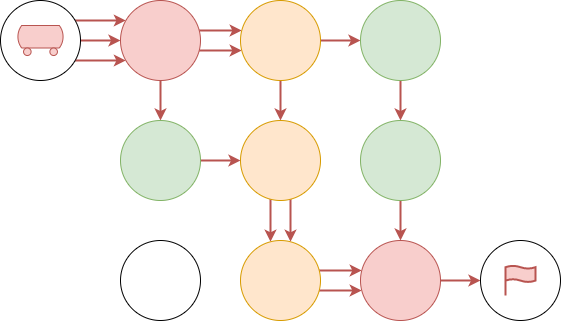
\includegraphics[width=\widthimg]{img/colored_heatmap.drawio.png}
\end{figure}

Furthermore, we formulate the following assumption \textit{``having a heatmap (global or agent one) that have the lowest sum of \(\phi\) and the lowest maximum \(\phi\) possible is desirable''} do not sound like a costly assumption. Given this assumption, we can then order different \(\gamma\) or \(\tau\) heatmaps. It of course, necessitate that the assumption is true, which may be (partially) decided with experiments.   


\subsection{Heatmap for subgraph}

\subsubsection{Straightforward solving}

In merging section~\ref{sec:merging}, we introduce ``straightforward solving'' which describe the case where we can find a combination of paths in \(\tau\) where a valid conflict-free set of paths can be found. However the process of picking these paths may be costly due to the exponential numbers of combination. However we can use heatmap as a preprocessing work; from a global heatmap, we can directly tell from the paths if a straightforward solving is not possible if, with \(|A| > 1\), for every vertices \(v\) in the heatmap, the following equation is true \( \Phi(v) > \sum{(a | v \in \gamma_a)} / |A|\). (Is the reciproque true ?) The following figure~\ref{img:heatmap_sf_solving} shows an example where the straightforward solving is decided from the heatmap; the orange vertex as a \(\Phi\) value superior to \(\sum{a | v \in \gamma_a} / |A| = 3/4 = 0.75\). On the other side, the figure~\ref{img:heatmap_sf_solving_possible} show the opposite case.

\begin{figure}[H]
  \centering
  \caption{Example of instance that is not possible to use straightforward solving}\label{img:heatmap_sf_solving}
  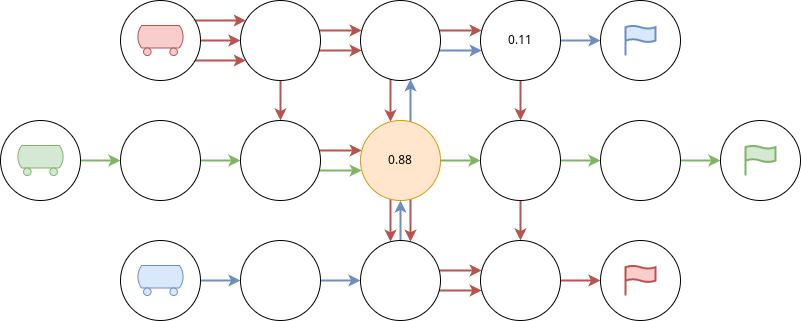
\includegraphics[width=\widthimg]{img/heatmap_sf_solving.drawio.png}
\end{figure}

\begin{figure}[H]
  \centering
  \caption{Example of instance that straightforward solving is at least undetermined}\label{img:heatmap_sf_solving_possible}
  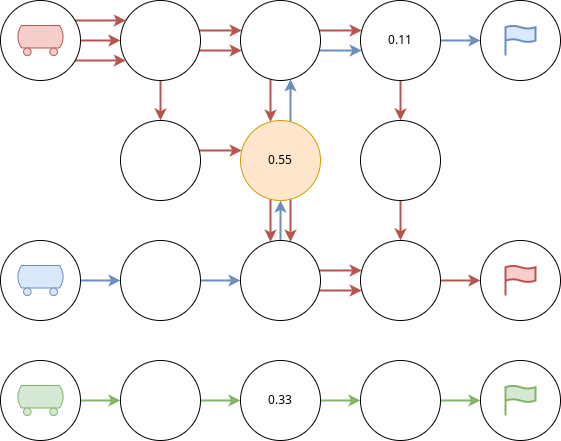
\includegraphics[width=\widthimg]{img/heatmap_sf_solving_possible.drawio.png}
\end{figure}


\subsubsection{Pruning the subgraph}


\subsection{Heatmap as a solving strategy}


\subsubsection{Misc}



\begin{itemize}
  \item X Can help for making \(\tau\) ; The way we define \(\phi\) can be an objective function; trying to minimize the sum of every \(\phi\) 
  \item Comparing \(\tau\) ; It seems that it is a visual and easy way to compare two different \(\tau\), compare to other properties of paths that we defined, this one seems the most appropriate for comparison.
  \item Can help on the decision if the straight forward resolution is possible.
  \item Helping for the subgraph subgraph; we can remove part of the subgraph for some agent where the global heat indicator is high and sees if ot relax the problem or not (keeping a connected subgraph). It can also probably provide information on which vertex could be added instead
  \item Solving by Guiding the agent
  \item Suit easily for robustness
\end{itemize}



Straightforward resolution refer to the fact that among all path in \(\tau\), we can find a combination of paths (1 for each agent) that is an actual solution for the problem. (explaining what is the process)


Guiding the agent

